\section{Results}
\label{sec:results}
Because the men would hang around the corner on windy days \cite{dresses}, a windy day was simulated with a wind speed of 9 $ms^{-1}$. To get a relatively accurate simulation, a iteration convergence of $1\cdot10^{-4}$ was recommended to us. \\\
\indent %
In order to adequately judge the wind around the building, an overview is created by plotting the streamlines at 3 different heights. These are shown at the bottom(figure \ref{fig:streamlinesbottom}), around the middle(figure \ref{fig:streamlinesmid}) and at the top(figure \ref{fig:streamlinestop}) of the Flatiron building and can be found in appendix \ref{sec:streamlines} \\
\indent %
To check if women's ankles would really show, a plot of the velocity in the z-direction, the pressure and the turbulent kinetic energy were made at a height of 1.37 meter (this was the lowest the program could go). These a shown, respectively, in figures \ref{fig:zvelocity}, \ref{fig:zpressure} and \ref{fig:zenergy}. \\
\begin{figure}[h!]
\centering
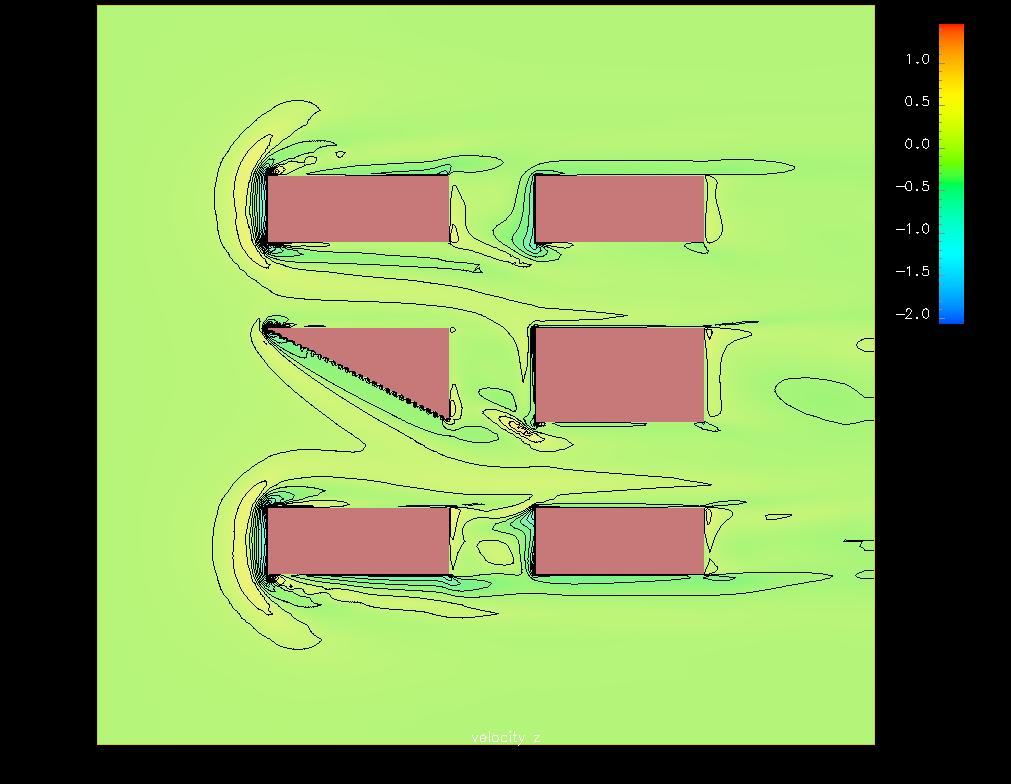
\includegraphics[width = \textwidth]{zvelocity.png}
\caption{Velocity in the z-direction around the Flatiron building at z=1.37 m}
\label{fig:zvelocity}
\end{figure}\\
\begin{figure}[h!]
\centering
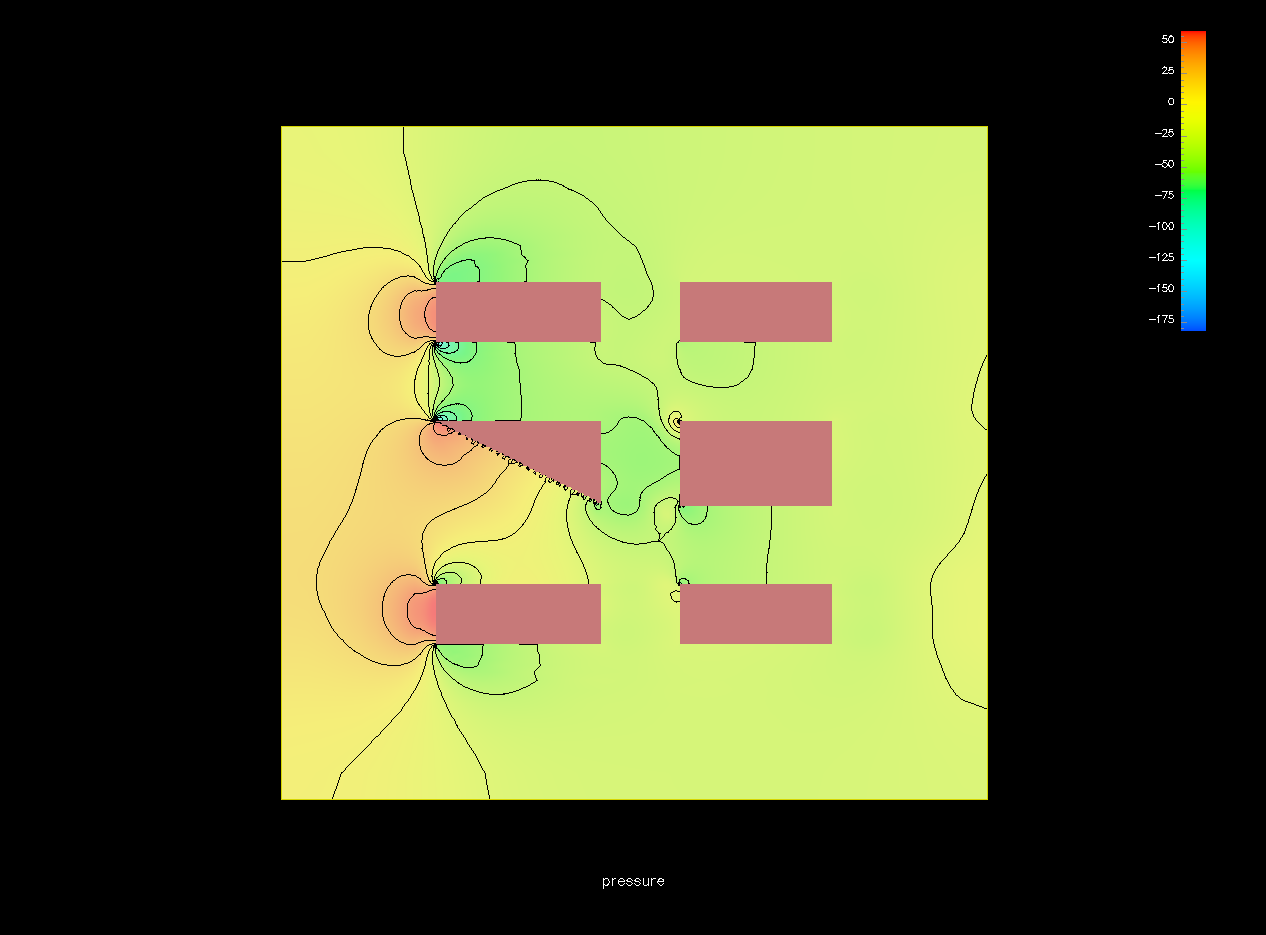
\includegraphics[width = \textwidth]{zpressure.png}
\caption{Pressure distribution(in Pa) around the Flatiron building at z=1.37 m}
\label{fig:zpressure}
\end{figure}\\
\begin{figure}[h!]
\centering
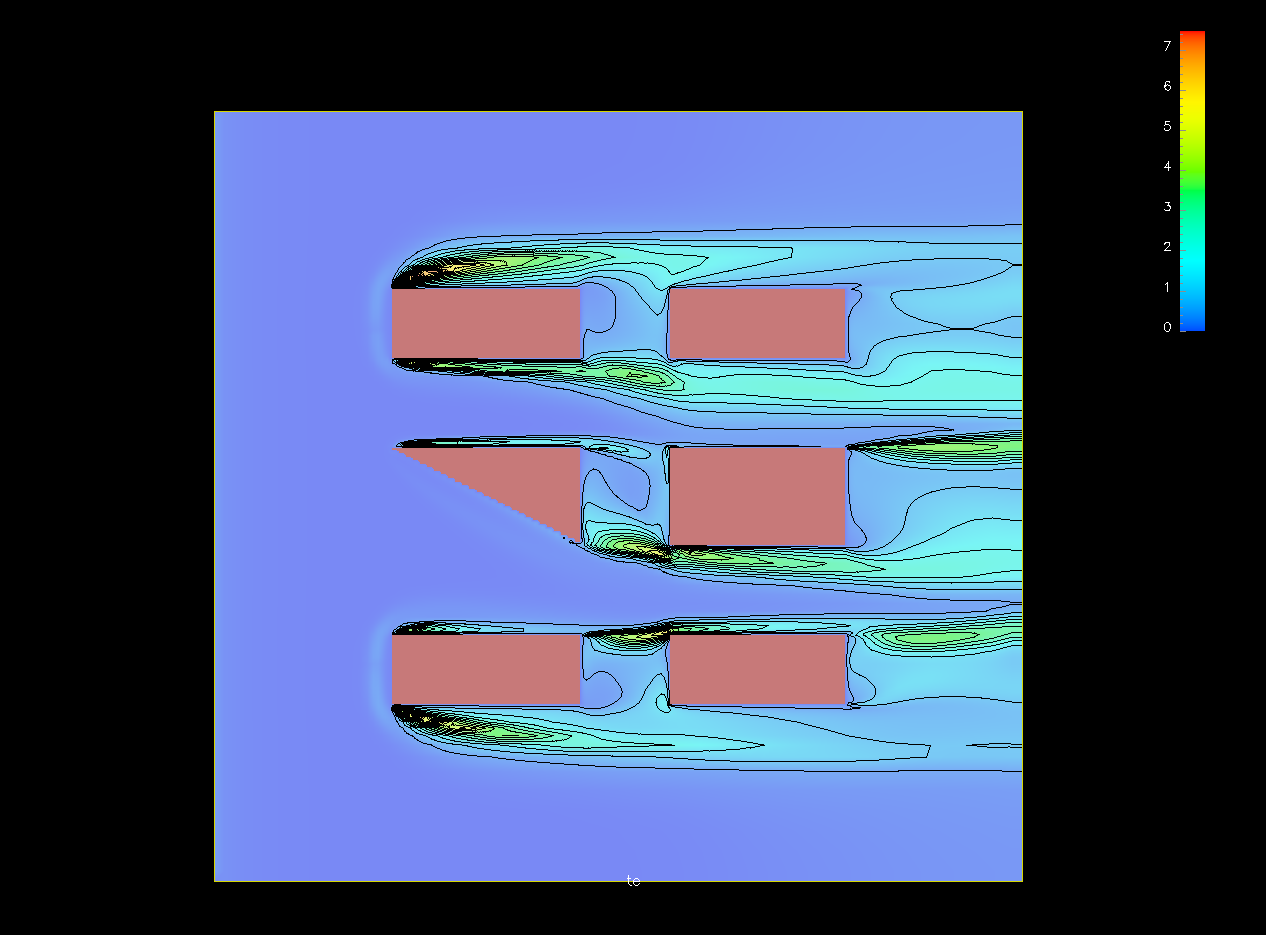
\includegraphics[width = \textwidth]{zenergy.png}
\caption{Turbulent kinetic energy(in $m^2s^{-2}$) around the Flatiron building at z=1.37 m}
\label{fig:zenergy}
\end{figure}\\
What is most interesting about the Flatiron building is the way it diverges the air. As seen in figure \ref{fig:zenergy}, there is barely any turbulence at the tip of the Flatiron building (a maximum of $2~m^2s^{-2}$) while at the other most upfront buildings, around the corners there is up to $7~m^2s^{-2}$. At the widest point of the Flatiron building, there is a lot of turbulent kinetic energy, most likely due to the wind hitting the edge of the building just behind that. This is also shown in figure \ref{fig:zpressure}, where the pressure builds up at that same corner. This rise in pressure and turbulent energy creates a small updraft, seen in \ref{fig:zvelocity}.\\
\indent %
Another remarkable thing is that the turbulent kinetic energy at the short side of the Flatiron building is lower than at the long side. It is suspected that this is because of the flow of air that goes into the street behind the Flatiron building. That this flow from the short side into the street and not from the long side can be seen in figure \ref{fig:streamlinesbottom}, where you see one streamline duck behind the building. This effect is more visible in figures \ref{fig:streamlinesmid} and \ref{fig:streamlinestop} where it is seen that at different heights, the wind from the shorter side of the Flatiron building ducks behind building, while the wind that comes from the longer side doesn\'t. 